\section{Patrón de Diseño Proxy} 
\textbf {1.    ¿Qué es el Patrón Proxy?}
\textbf{}\\
El patrón Proxy proporciona un objeto intermediario entre el cliente y el objeto a utilizar, que permite configurar ciertas características (como el acceso) sin necesidad de modificar la clase original.
\begin{flushleft}
\begin{center}
	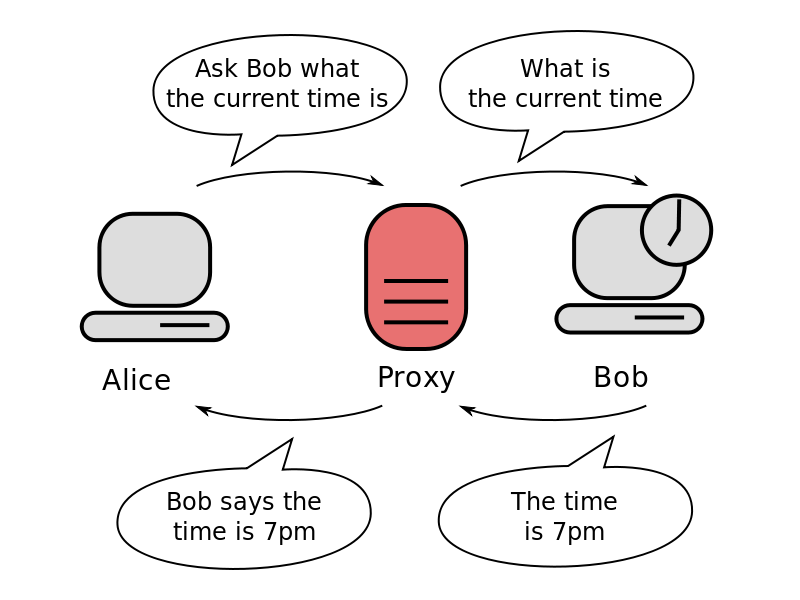
\includegraphics[width=10cm]{./Imagenes/proxy1} 
	\end{center}
\begin{itemize}
	\item Por ejemplo:
Si tenemos muchos objetos imagen en un documento, se tardaría mucho tiempo en abrir el documento al cargar las imágenes de disco. Para evitarlo podemos sustituir los objetos imagen por objetos proxyImagen, con el mismo interfaz, pero que solamente cargan la imagen cuando se va a visualizar.

\textbf {2.	Tipos de Patrón Proxy}
\textbf{}\\
Existen varios tipos de Proxy que realizan distintos tipos de tareas: Proxy Remoto, Proxy Virtual, Proxy de Protección.

\item	\textbf {Proxy Remoto:} Se comporta como un representante local de un objeto, al realizar esto lo que hace es abstraer toda la “conversación” entre “dos” y de esta forma la comunicación entre el cliente y el objeto remoto es más fácil gastando menos recursos.
\item	\textbf {Proxy Virtual:} Lo que hace el proxy virtual es instanciar objetos cuyo costo computacional es muy elevado.

 \item	\textbf {Proxy Protección:} Lo único que hace es establecer el control de acceso a un objeto dependiendo de los permisos o reglas de autorización.


\textbf {3.	Estructura del Patrón Proxy}
\textbf{}\\

\textbf {3.1.	Clasificación}
\textbf{}\\
\item	\textbf {Patrón estructural:} Ya que define la forma en cómo se organizan los objetos y las dependencias que tiene entre ellos.
\textbf{}\\
\textbf {3.2.	Aplicaciones}
\textbf{}\\

\item Útil cuando se desea retrasar la instanciación de un objeto hasta que sea necesario usarlo (optimiza operaciones costosas: invocar imagen). 
\item Proporciona un representante local de un objeto situado en otro espacio de direcciones (Proxy remoto o “Embajador”). 
\item Uso en sistemas concurrentes, mediante cerrojo, controlando el acceso al objeto original. 
\item Puede utilizarse como un sustituto de un simple puntero, que lleva a cabo operaciones adicionales cuando se accede a un objeto (contar el número de referencias a un objeto real).

\textbf{}\\
\textbf {3.3.	Consecuencias}
\textbf{}\\
\item Un proxy puede ocultar el hecho de que un objeto reside en un espacio de direcciones diferente (proxy remoto). 
\item Puede llevar a cabo optimizaciones tales como crear un objeto por encargo (invocar imagen). 
\item Permiten realizar tareas de mantenimiento adicionales cuando se accede a un objeto (Proxy de protección y de referencias inteligentes).
\item Se introduce un nivel de indirección al acceder al objeto.
\item Se consigue una administración transparente de los servicios del objeto real. 
\begin{center}
\textbf {Representación UML}
\end{center}
\begin{center}

	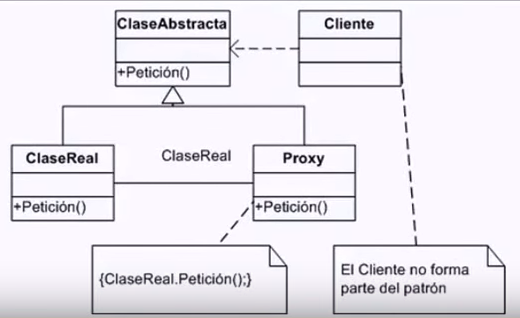
\includegraphics[width=10cm]{./Imagenes/proxy2} 
	\end{center}

\textbf{}\\
\textbf {3.4.	Participantes}
\textbf{}\\


\item	\textbf {Sujeto:} Define la interfaz común para el RealSubject y el Proxy, de modo que pueda usarse un Proxy en cualquier sitio en el que se espere un RealSubject.
\textbf{}\\
\item	\textbf {RealSubject:} Define el objeto real representado.
\textbf{}\\
\item	\textbf {Proxy:}
\textbf{}\\
Mantiene una referencia que permite al Proxy acceder al objeto real. 
Proporciona una interfaz idéntica a la del sujeto, de manera que un Proxy pueda ser sustituido por el sujeto real. 
Controla el acceso al sujeto real, y puede ser responsable de su creación y borrado.
\textbf{}\\
\textbf{}\\

\textbf {4.	Ejemplos UML}

\item	\textbf {Diagrama UML}
\textbf{}\\
Un ejemplo típico de aplicación del patrón proxy es el de un editor de documentos. El editor podrá incluir imágenes y dibujos complejos, y se plantea el problema de recuperar todos estos costosos objetos cada vez que se abre el documento. La aplicación del patrón proxy soluciona el problema definiendo un "representante", que ocupe su lugar, hasta que sea necesario cargarlos.
\begin{center}

	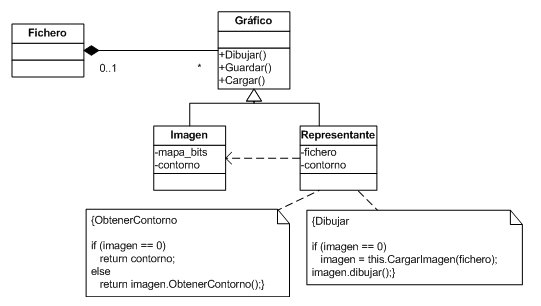
\includegraphics[width=10cm]{./Imagenes/proxy3} 
	\end{center}



\textbf {5.	Ejemplos de Implementación sin Proxy y/o con Proxy}

\item	\textbf {Sin Proxy}

\begin{center}

	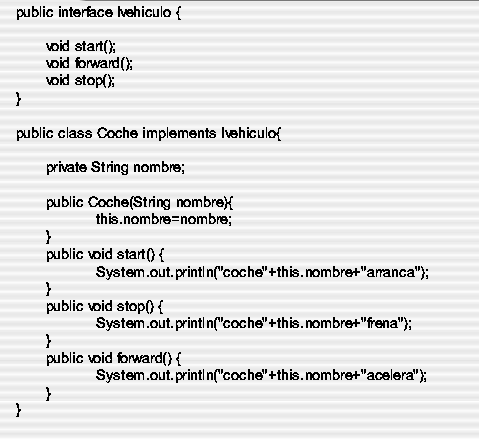
\includegraphics[width=10cm]{./Imagenes/proxy4} 
	\end{center}
\begin{center}
\textbf{}\\
	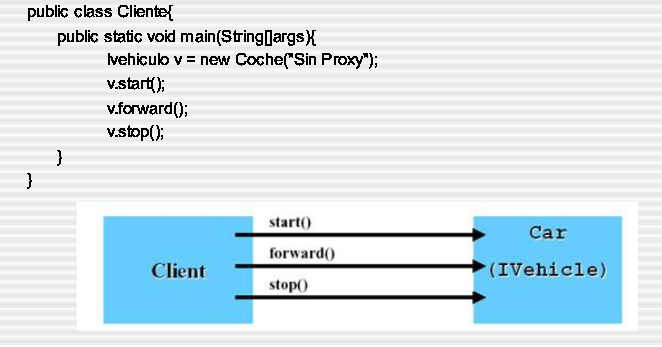
\includegraphics[width=10cm]{./Imagenes/proxy5} 
	\end{center}


\item	\textbf {Con Proxy}

\begin{center}

	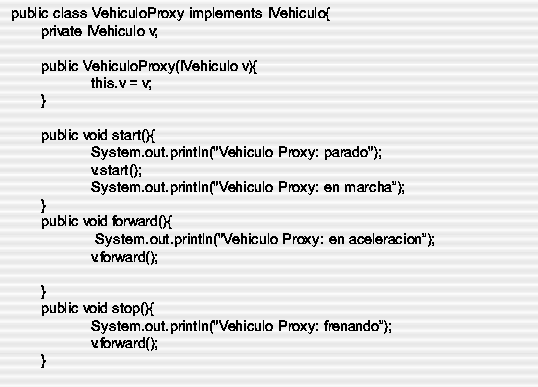
\includegraphics[width=10cm]{./Imagenes/proxy6} 
	\end{center}
\begin{center}
\textbf{}\\
	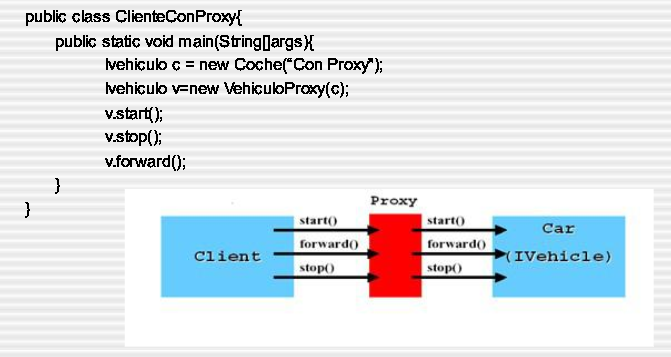
\includegraphics[width=10cm]{./Imagenes/proxy7} 
	\end{center}



\textbf {6.	Conclusiones}

\item	\textbf {No Proxy:} El cliente interactúa directamente con los métodos definidos en la interface 

\item	\textbf {Proxy:} Se encuentra entre la interfaz y la implementación e intercepta las llamadas a los métodos. La intención del Proxy es controlar el acceso al objeto deseado, además de mejorar la funcionalidad del mismo 


	

\end{itemize} 


\end{flushleft}